\definecolor{tblue}{RGB}{61,142,221}
\definecolor{torange}{RGB}{253,143,41}
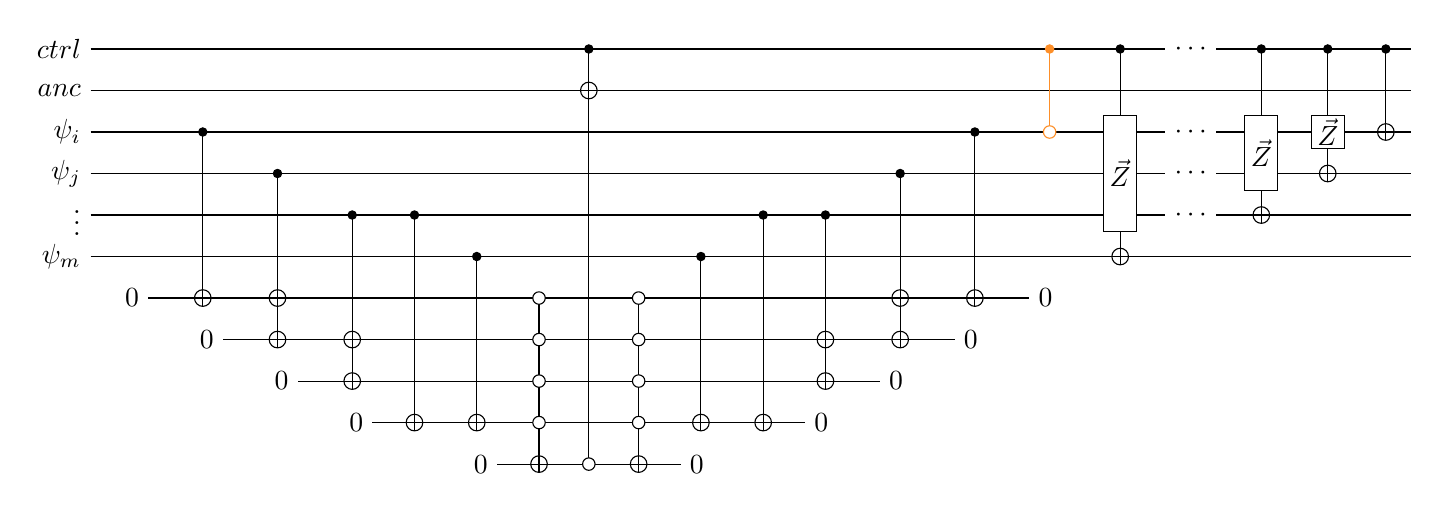
\begin{tikzpicture}[scale=1.000000,x=1pt,y=1pt]
\filldraw[color=white] (0.000000, -7.500000) rectangle (477.000000, 157.500000);
% Drawing wires
% Line 4: ctrl W ctrl
\draw[color=black] (0.000000,150.000000) -- (477.000000,150.000000);
\draw[color=black] (0.000000,150.000000) node[left] {$ctrl$};
% Line 5: anc W anc
\draw[color=black] (0.000000,135.000000) -- (477.000000,135.000000);
\draw[color=black] (0.000000,135.000000) node[left] {$anc$};
% Line 6: a W \psi_i
\draw[color=black] (0.000000,120.000000) -- (477.000000,120.000000);
\draw[color=black] (0.000000,120.000000) node[left] {$\psi_i$};
% Line 7: b W \psi_j
\draw[color=black] (0.000000,105.000000) -- (477.000000,105.000000);
\draw[color=black] (0.000000,105.000000) node[left] {$\psi_j$};
% Line 8: c W \vdots
\draw[color=black] (0.000000,90.000000) -- (477.000000,90.000000);
\draw[color=black] (0.000000,90.000000) node[left] {$\vdots$};
% Line 9: f W \psi_m
\draw[color=black] (0.000000,75.000000) -- (477.000000,75.000000);
\draw[color=black] (0.000000,75.000000) node[left] {$\psi_m$};
% Line 10: c0 W 0 0
\draw[color=black] (13.500000,60.000000) -- (346.500000,60.000000);
% Line 11: c1 W 0 0
\draw[color=black] (40.500000,45.000000) -- (319.500000,45.000000);
% Line 12: c2 W 0 0
\draw[color=black] (67.500000,30.000000) -- (292.500000,30.000000);
% Line 13: 1 W 0 0
\draw[color=black] (94.500000,15.000000) -- (265.500000,15.000000);
% Line 14: c3 W 0 0
\draw[color=black] (139.500000,0.000000) -- (220.500000,0.000000);
% Done with wires; drawing gates
% Line 16: c0 START
\draw[color=black] (21.000000,60.000000) node[fill=white,left,minimum height=15.000000pt,minimum width=15.000000pt,inner sep=0pt] {\phantom{$0$}};
\draw[color=black] (21.000000,60.000000) node[left] {$0$};
% Line 17: a +c0
\draw (40.500000,120.000000) -- (40.500000,60.000000);
\filldraw (40.500000, 120.000000) circle(1.500000pt);
\begin{scope}
\draw[fill=white] (40.500000, 60.000000) circle(3.000000pt);
\clip (40.500000, 60.000000) circle(3.000000pt);
\draw (37.500000, 60.000000) -- (43.500000, 60.000000);
\draw (40.500000, 57.000000) -- (40.500000, 63.000000);
\end{scope}
% Line 18: c1 START
\draw[color=black] (48.000000,45.000000) node[fill=white,left,minimum height=15.000000pt,minimum width=15.000000pt,inner sep=0pt] {\phantom{$0$}};
\draw[color=black] (48.000000,45.000000) node[left] {$0$};
% Line 19: b +c0 +c1
\draw (67.500000,105.000000) -- (67.500000,45.000000);
\filldraw (67.500000, 105.000000) circle(1.500000pt);
\begin{scope}
\draw[fill=white] (67.500000, 60.000000) circle(3.000000pt);
\clip (67.500000, 60.000000) circle(3.000000pt);
\draw (64.500000, 60.000000) -- (70.500000, 60.000000);
\draw (67.500000, 57.000000) -- (67.500000, 63.000000);
\end{scope}
\begin{scope}
\draw[fill=white] (67.500000, 45.000000) circle(3.000000pt);
\clip (67.500000, 45.000000) circle(3.000000pt);
\draw (64.500000, 45.000000) -- (70.500000, 45.000000);
\draw (67.500000, 42.000000) -- (67.500000, 48.000000);
\end{scope}
% Line 20: c2 START
\draw[color=black] (75.000000,30.000000) node[fill=white,left,minimum height=15.000000pt,minimum width=15.000000pt,inner sep=0pt] {\phantom{$0$}};
\draw[color=black] (75.000000,30.000000) node[left] {$0$};
% Line 21: c +c1 +c2
\draw (94.500000,90.000000) -- (94.500000,30.000000);
\filldraw (94.500000, 90.000000) circle(1.500000pt);
\begin{scope}
\draw[fill=white] (94.500000, 45.000000) circle(3.000000pt);
\clip (94.500000, 45.000000) circle(3.000000pt);
\draw (91.500000, 45.000000) -- (97.500000, 45.000000);
\draw (94.500000, 42.000000) -- (94.500000, 48.000000);
\end{scope}
\begin{scope}
\draw[fill=white] (94.500000, 30.000000) circle(3.000000pt);
\clip (94.500000, 30.000000) circle(3.000000pt);
\draw (91.500000, 30.000000) -- (97.500000, 30.000000);
\draw (94.500000, 27.000000) -- (94.500000, 33.000000);
\end{scope}
% Line 22: 1 START
\draw[color=black] (102.000000,15.000000) node[fill=white,left,minimum height=15.000000pt,minimum width=15.000000pt,inner sep=0pt] {\phantom{$0$}};
\draw[color=black] (102.000000,15.000000) node[left] {$0$};
% Line 23: c +1
\draw (117.000000,90.000000) -- (117.000000,15.000000);
\filldraw (117.000000, 90.000000) circle(1.500000pt);
\begin{scope}
\draw[fill=white] (117.000000, 15.000000) circle(3.000000pt);
\clip (117.000000, 15.000000) circle(3.000000pt);
\draw (114.000000, 15.000000) -- (120.000000, 15.000000);
\draw (117.000000, 12.000000) -- (117.000000, 18.000000);
\end{scope}
% Line 24: f +1
\draw (139.500000,75.000000) -- (139.500000,15.000000);
\filldraw (139.500000, 75.000000) circle(1.500000pt);
\begin{scope}
\draw[fill=white] (139.500000, 15.000000) circle(3.000000pt);
\clip (139.500000, 15.000000) circle(3.000000pt);
\draw (136.500000, 15.000000) -- (142.500000, 15.000000);
\draw (139.500000, 12.000000) -- (139.500000, 18.000000);
\end{scope}
% Line 26: c3 START
\draw[color=black] (147.000000,0.000000) node[fill=white,left,minimum height=15.000000pt,minimum width=15.000000pt,inner sep=0pt] {\phantom{$0$}};
\draw[color=black] (147.000000,0.000000) node[left] {$0$};
% Line 27: -c0 -c1 -c2 -1 +c3
\draw (162.000000,60.000000) -- (162.000000,0.000000);
\draw[fill=white] (162.000000, 60.000000) circle(2.250000pt);
\draw[fill=white] (162.000000, 45.000000) circle(2.250000pt);
\draw[fill=white] (162.000000, 30.000000) circle(2.250000pt);
\draw[fill=white] (162.000000, 15.000000) circle(2.250000pt);
\begin{scope}
\draw[fill=white] (162.000000, 0.000000) circle(3.000000pt);
\clip (162.000000, 0.000000) circle(3.000000pt);
\draw (159.000000, 0.000000) -- (165.000000, 0.000000);
\draw (162.000000, -3.000000) -- (162.000000, 3.000000);
\end{scope}
% Line 28: ctrl -c3 +anc
\draw (180.000000,150.000000) -- (180.000000,0.000000);
\filldraw (180.000000, 150.000000) circle(1.500000pt);
\draw[fill=white] (180.000000, 0.000000) circle(2.250000pt);
\begin{scope}
\draw[fill=white] (180.000000, 135.000000) circle(3.000000pt);
\clip (180.000000, 135.000000) circle(3.000000pt);
\draw (177.000000, 135.000000) -- (183.000000, 135.000000);
\draw (180.000000, 132.000000) -- (180.000000, 138.000000);
\end{scope}
% Line 29: -c0 -c1 -c2 -1 +c3
\draw (198.000000,60.000000) -- (198.000000,0.000000);
\draw[fill=white] (198.000000, 60.000000) circle(2.250000pt);
\draw[fill=white] (198.000000, 45.000000) circle(2.250000pt);
\draw[fill=white] (198.000000, 30.000000) circle(2.250000pt);
\draw[fill=white] (198.000000, 15.000000) circle(2.250000pt);
\begin{scope}
\draw[fill=white] (198.000000, 0.000000) circle(3.000000pt);
\clip (198.000000, 0.000000) circle(3.000000pt);
\draw (195.000000, 0.000000) -- (201.000000, 0.000000);
\draw (198.000000, -3.000000) -- (198.000000, 3.000000);
\end{scope}
% Line 30: c3 END
\draw[color=black] (213.000000,0.000000) node[fill=white,right,minimum height=15.000000pt,minimum width=15.000000pt,inner sep=0pt] {\phantom{$0$}};
\draw[color=black] (213.000000,0.000000) node[right] {$0$};
% Line 32: f +1
\draw (220.500000,75.000000) -- (220.500000,15.000000);
\filldraw (220.500000, 75.000000) circle(1.500000pt);
\begin{scope}
\draw[fill=white] (220.500000, 15.000000) circle(3.000000pt);
\clip (220.500000, 15.000000) circle(3.000000pt);
\draw (217.500000, 15.000000) -- (223.500000, 15.000000);
\draw (220.500000, 12.000000) -- (220.500000, 18.000000);
\end{scope}
% Line 33: c +1
\draw (243.000000,90.000000) -- (243.000000,15.000000);
\filldraw (243.000000, 90.000000) circle(1.500000pt);
\begin{scope}
\draw[fill=white] (243.000000, 15.000000) circle(3.000000pt);
\clip (243.000000, 15.000000) circle(3.000000pt);
\draw (240.000000, 15.000000) -- (246.000000, 15.000000);
\draw (243.000000, 12.000000) -- (243.000000, 18.000000);
\end{scope}
% Line 34: 1 END
\draw[color=black] (258.000000,15.000000) node[fill=white,right,minimum height=15.000000pt,minimum width=15.000000pt,inner sep=0pt] {\phantom{$0$}};
\draw[color=black] (258.000000,15.000000) node[right] {$0$};
% Line 35: c +c1 +c2
\draw (265.500000,90.000000) -- (265.500000,30.000000);
\filldraw (265.500000, 90.000000) circle(1.500000pt);
\begin{scope}
\draw[fill=white] (265.500000, 45.000000) circle(3.000000pt);
\clip (265.500000, 45.000000) circle(3.000000pt);
\draw (262.500000, 45.000000) -- (268.500000, 45.000000);
\draw (265.500000, 42.000000) -- (265.500000, 48.000000);
\end{scope}
\begin{scope}
\draw[fill=white] (265.500000, 30.000000) circle(3.000000pt);
\clip (265.500000, 30.000000) circle(3.000000pt);
\draw (262.500000, 30.000000) -- (268.500000, 30.000000);
\draw (265.500000, 27.000000) -- (265.500000, 33.000000);
\end{scope}
% Line 36: c2 END
\draw[color=black] (285.000000,30.000000) node[fill=white,right,minimum height=15.000000pt,minimum width=15.000000pt,inner sep=0pt] {\phantom{$0$}};
\draw[color=black] (285.000000,30.000000) node[right] {$0$};
% Line 37: b +c0 +c1
\draw (292.500000,105.000000) -- (292.500000,45.000000);
\filldraw (292.500000, 105.000000) circle(1.500000pt);
\begin{scope}
\draw[fill=white] (292.500000, 60.000000) circle(3.000000pt);
\clip (292.500000, 60.000000) circle(3.000000pt);
\draw (289.500000, 60.000000) -- (295.500000, 60.000000);
\draw (292.500000, 57.000000) -- (292.500000, 63.000000);
\end{scope}
\begin{scope}
\draw[fill=white] (292.500000, 45.000000) circle(3.000000pt);
\clip (292.500000, 45.000000) circle(3.000000pt);
\draw (289.500000, 45.000000) -- (295.500000, 45.000000);
\draw (292.500000, 42.000000) -- (292.500000, 48.000000);
\end{scope}
% Line 38: c1 END
\draw[color=black] (312.000000,45.000000) node[fill=white,right,minimum height=15.000000pt,minimum width=15.000000pt,inner sep=0pt] {\phantom{$0$}};
\draw[color=black] (312.000000,45.000000) node[right] {$0$};
% Line 39: a +c0
\draw (319.500000,120.000000) -- (319.500000,60.000000);
\filldraw (319.500000, 120.000000) circle(1.500000pt);
\begin{scope}
\draw[fill=white] (319.500000, 60.000000) circle(3.000000pt);
\clip (319.500000, 60.000000) circle(3.000000pt);
\draw (316.500000, 60.000000) -- (322.500000, 60.000000);
\draw (319.500000, 57.000000) -- (319.500000, 63.000000);
\end{scope}
% Line 40: c0 END
\draw[color=black] (339.000000,60.000000) node[fill=white,right,minimum height=15.000000pt,minimum width=15.000000pt,inner sep=0pt] {\phantom{$0$}};
\draw[color=black] (339.000000,60.000000) node[right] {$0$};
% Line 44: ctrl -a color=torange
\begin{scope}[color=torange]
\draw (346.500000,150.000000) -- (346.500000,120.000000);
\filldraw (346.500000, 150.000000) circle(1.500000pt);
\draw[fill=white] (346.500000, 120.000000) circle(2.250000pt);
\end{scope}
% Line 46: a b c G $\vec{Z}$ ctrl +f
\draw (372.000000,150.000000) -- (372.000000,75.000000);
\begin{scope}
\draw[fill=white] (372.000000, 105.000000) +(-45.000000:8.485281pt and 29.698485pt) -- +(45.000000:8.485281pt and 29.698485pt) -- +(135.000000:8.485281pt and 29.698485pt) -- +(225.000000:8.485281pt and 29.698485pt) -- cycle;
\clip (372.000000, 105.000000) +(-45.000000:8.485281pt and 29.698485pt) -- +(45.000000:8.485281pt and 29.698485pt) -- +(135.000000:8.485281pt and 29.698485pt) -- +(225.000000:8.485281pt and 29.698485pt) -- cycle;
\draw (372.000000, 105.000000) node {$\vec{Z}$};
\end{scope}
\filldraw (372.000000, 150.000000) circle(1.500000pt);
\begin{scope}
\draw[fill=white] (372.000000, 75.000000) circle(3.000000pt);
\clip (372.000000, 75.000000) circle(3.000000pt);
\draw (369.000000, 75.000000) -- (375.000000, 75.000000);
\draw (372.000000, 72.000000) -- (372.000000, 78.000000);
\end{scope}
% Line 47: ctrl a b c LABEL ...
\draw[color=black] (397.500000, 150.000000) node [fill=white] {$\cdots$};
\draw[color=black] (397.500000, 120.000000) node [fill=white] {$\cdots$};
\draw[color=black] (397.500000, 105.000000) node [fill=white] {$\cdots$};
\draw[color=black] (397.500000, 90.000000) node [fill=white] {$\cdots$};
% Line 48: a b G $\vec{Z}$ ctrl +c
\draw (423.000000,150.000000) -- (423.000000,90.000000);
\begin{scope}
\draw[fill=white] (423.000000, 112.500000) +(-45.000000:8.485281pt and 19.091883pt) -- +(45.000000:8.485281pt and 19.091883pt) -- +(135.000000:8.485281pt and 19.091883pt) -- +(225.000000:8.485281pt and 19.091883pt) -- cycle;
\clip (423.000000, 112.500000) +(-45.000000:8.485281pt and 19.091883pt) -- +(45.000000:8.485281pt and 19.091883pt) -- +(135.000000:8.485281pt and 19.091883pt) -- +(225.000000:8.485281pt and 19.091883pt) -- cycle;
\draw (423.000000, 112.500000) node {$\vec{Z}$};
\end{scope}
\filldraw (423.000000, 150.000000) circle(1.500000pt);
\begin{scope}
\draw[fill=white] (423.000000, 90.000000) circle(3.000000pt);
\clip (423.000000, 90.000000) circle(3.000000pt);
\draw (420.000000, 90.000000) -- (426.000000, 90.000000);
\draw (423.000000, 87.000000) -- (423.000000, 93.000000);
\end{scope}
% Line 49: a G $\vec{Z}$ ctrl +b
\draw (447.000000,150.000000) -- (447.000000,105.000000);
\begin{scope}
\draw[fill=white] (447.000000, 120.000000) +(-45.000000:8.485281pt and 8.485281pt) -- +(45.000000:8.485281pt and 8.485281pt) -- +(135.000000:8.485281pt and 8.485281pt) -- +(225.000000:8.485281pt and 8.485281pt) -- cycle;
\clip (447.000000, 120.000000) +(-45.000000:8.485281pt and 8.485281pt) -- +(45.000000:8.485281pt and 8.485281pt) -- +(135.000000:8.485281pt and 8.485281pt) -- +(225.000000:8.485281pt and 8.485281pt) -- cycle;
\draw (447.000000, 120.000000) node {$\vec{Z}$};
\end{scope}
\filldraw (447.000000, 150.000000) circle(1.500000pt);
\begin{scope}
\draw[fill=white] (447.000000, 105.000000) circle(3.000000pt);
\clip (447.000000, 105.000000) circle(3.000000pt);
\draw (444.000000, 105.000000) -- (450.000000, 105.000000);
\draw (447.000000, 102.000000) -- (447.000000, 108.000000);
\end{scope}
% Line 50: ctrl +a
\draw (468.000000,150.000000) -- (468.000000,120.000000);
\filldraw (468.000000, 150.000000) circle(1.500000pt);
\begin{scope}
\draw[fill=white] (468.000000, 120.000000) circle(3.000000pt);
\clip (468.000000, 120.000000) circle(3.000000pt);
\draw (465.000000, 120.000000) -- (471.000000, 120.000000);
\draw (468.000000, 117.000000) -- (468.000000, 123.000000);
\end{scope}
% Done with gates; drawing ending labels
% Done with ending labels; drawing cut lines and comments
% Done with comments
\end{tikzpicture}
